\documentclass[letterpaper]{article}

% AAAI-27 author-kit baseline. Keep submission mode until the anonymous-review
% process is complete.
\usepackage[submission]{aaai2027}
\usepackage[hyphens]{url}
\usepackage{graphicx}
\urlstyle{rm}
\def\UrlFont{\rm}
\usepackage{natbib}
\usepackage{caption}
\usepackage{booktabs}
\frenchspacing
\pdfinfo{/TemplateVersion (2027.1)}

\setcounter{secnumdepth}{2}

% Working title retained after the P9 whole-paper audit. Final human approval
% remains TODO-HUMAN G-HUM-01.
\title{CliniCause: Constructing Reusable Causal-Analysis Datasets from Irregular ICU Records}
\author{Anonymous Submission}
\affiliations{}

\begin{document}
\maketitle

\begin{abstract}
Reusable causal analysis of heterogeneous, irregular intensive-care records
requires explicit constructs, cohort boundaries, adjustment assumptions, and
provenance that prediction-ready sequences do not provide. We present
CliniCause, two validated causal-analysis datasets built from MIMIC-III and
PhysioNet 2012. The resources contain 26,845 and 7,993 analysis records with
nine and ten admitted proxy-state exposures, respectively, linked to
in-hospital mortality, observed covariates, dataset-specific causal-graph
metadata, and provenance. An evidence-tracked pipeline combines deterministic
proxy rules with annotations from four irregular-time-series models and
enforces schema, cohort, artifact, and provenance contracts; a design-time LLM
proposes candidates but does not process patient records or estimate effects.
On archived predictive point metrics, STraTS led all four MIMIC-III metrics and
GRU-D led all four PhysioNet metrics. Across 19 prespecified dataset--exposure
comparisons, the two double-machine-learning estimators agreed in direction for
19/19, while CausalPFN joined them in 18/19; PhysioNet shock was the sole
all-estimator exception. These observational, proxy-based results do not
establish clinical effects or causal identification. They show that CliniCause
supports reusable, inspectable analysis and that estimator triangulation can
expose both stable directional patterns and informative disagreements across
heterogeneous ICU resources.
\end{abstract}

\section{Introduction}

Intensive-care records combine measurements, care processes, and outcomes
observed at unequal frequencies and times. Their missingness can reflect both
patient state and clinical workflow
\cite{sun_2026_review_irregular_medical_timeseries,
lipton_kale_wetzel_2016_missingness_rnns}. Causal analysis therefore requires
more than a prediction-ready sequence: it needs explicit analysis units,
exposures, outcomes, covariates, cohort boundaries, adjustment assumptions, and
provenance. Reconstructing these interfaces study by study makes silent changes
to constructs or cohorts hard to detect. Identifier conventions, measurement
availability, and preprocessing can alter which records reach analysis even
when studies begin from the same database. A reusable resource must therefore
preserve both variables and the lineage and assumptions that give them
analytical meaning.

ICU databases and benchmarks provide source records and prediction tasks
\cite{johnson2016mimiciii,silva2012physionet,
harutyunyan_2019_mimiciii_benchmark}; irregular-time-series models represent
sparse events or measurement gaps \cite{tipirneni2022strats,che2018grud};
electronic phenotyping and weak supervision turn clinical evidence or heuristics
into analytical labels \cite{banda_2018_electronic_phenotyping,
ratner_et_al_2016_data_programming}; and causal machine learning estimates
adjusted, potentially heterogeneous contrasts \cite{chernozhukov2018dml,
wager2018causalforest}. What remains difficult is their resource-level
integration: carrying replaceable proxy constructs from heterogeneous irregular
records through predictive annotation into graph-documented, estimator-ready
datasets with validation and provenance. Without that interface, targets,
exposures, adjustment variables, and populations may each be defensible yet
difficult to reuse or compare as one traceable scientific object.
The challenge is not simply to concatenate components, but to make every
handoff explicit enough that a construct, cohort, or adjustment decision can be
changed and audited without silently redefining the rest of the analysis.

CliniCause constructs two such resources from MIMIC-III and PhysioNet 2012
under a common interface while preserving dataset-specific semantics. Rules
define project-selected proxy states; four temporal models add predictive
annotations; and each resource joins aggregate proxy exposures to in-hospital
mortality, observed covariates, causal-graph adjustment metadata, cohort
identity, and provenance. A design-time LLM proposed candidates that were
project-selected and encoded as deterministic source before patient-level
execution. The datasets and estimates remain separate. Here, \emph{validated}
denotes construction and analytical integrity---aligned schemas, cohorts,
artifacts, provenance, and analytical use---not clinical construct validation
or causal identification.

The resources contain 26,845 MIMIC-III records with nine admitted exposures and
7,993 PhysioNet records with ten. STraTS led all four archived MIMIC-III point
metrics, whereas GRU-D led all four PhysioNet metrics. CausalForestDML and
LinearDML agreed in direction for 19/19 prespecified comparisons, CausalPFN
joined them in 18/19, and 55/57 original-versus-downsampled estimator
comparisons preserved direction.

Our contributions are: (1)~two reusable, validated causal-analysis datasets;
(2)~an evidence-tracked pipeline integrating deterministic proxies, temporal
prediction, causal-graph metadata, validation, provenance, and bounded
design-time LLM assistance; (3)~predictive and three-estimator characterization,
including 19/19 DML and 18/19 all-estimator directional agreement; and
(4)~interfaces for replacing proxies, temporal models, graphs, adjustment sets,
estimators, and robustness analyses without repeating upstream integration.
The hierarchy keeps the resources primary, their construction pipeline second,
and empirical analyses as demonstrations of utility.

\section{Related Work}

MIMIC-III provides heterogeneous critical-care records, while PhysioNet 2012
and the MIMIC-III benchmark define prediction tasks
\cite{johnson2016mimiciii,silva2012physionet,
harutyunyan_2019_mimiciii_benchmark}. GRU-D models informative missingness and
STraTS represents sparse time--variable--value events
\cite{che2018grud,tipirneni2022strats}; GRU and TCN supply recurrent and
convolutional baselines \cite{cho2014gru,bai2018tcn}. CliniCause uses these
model families to annotate explicit proxies for downstream causal analysis.
Unlike prediction benchmarks, the final object here includes exposure,
adjustment, cohort, and provenance interfaces for estimator comparison.
Thus temporal models are evaluated as annotation mechanisms inside a larger
resource contract rather than as mortality-prediction endpoints.

Electronic phenotyping spans inspectable rules and learned models
\cite{banda_2018_electronic_phenotyping}; data programming and Snorkel formalize
heuristic labeling sources \cite{ratner_et_al_2016_data_programming,
ratner_et_al_2020_snorkel}. CliniCause uses no trained label model: it preserves
dataset-specific deterministic definitions and applies a fixed majority vote
over one rule and four model sources, keeping construct lineage explicit. This
retains the inspectability of programmatic labeling while separating the fixed
aggregation from methods that learn source accuracy or dependence.
The resulting vote is consequently an implemented analytical construct, not an
estimate of diagnostic truth or annotator consensus.

Double machine learning accommodates flexible nuisance estimation through
orthogonal scores and cross-fitting \cite{chernozhukov2018dml}; causal and
generalized random forests model heterogeneous effects under their assumptions
\cite{wager2018causalforest,athey2019grf}. CausalPFN instead amortizes effect
estimation in a prior-data-fitted, in-context model trained on simulated
data-generating processes \cite{balazadeh2025causalpfn}. These methods provide
estimators, whereas CliniCause contributes the reusable exposure, outcome,
covariate, cohort, graph, adjustment, and provenance interfaces on which they
are compared. Estimator innovation alone does not supply a traceable clinical
analysis table or preserve the construct decisions that produced it.
CliniCause complements estimator research by holding these inputs and decisions
in an inspectable, dataset-specific resource boundary.

Medical LLM studies show capability alongside reliability gaps, and causal-graph
work treats LLM judgments as fallible priors
\cite{singhal_et_al_2023_llm_clinical_knowledge,
darvariu_et_al_2024_llm_causal_graph_priors}. CliniCause therefore restricts the
LLM to inspectable design proposals and leaves runtime authority to deterministic
source. Its contribution is the traceable integration of these otherwise
separate strands into two reusable causal-analysis resources; the LLM is a
bounded proposal mechanism rather than a clinical or estimation authority.
This division preserves the benefit of structured elicitation while leaving
both the accepted proposal and its deterministic implementation open to review.

\section{Constructing the CliniCause Datasets}
% P3 claim locations: C01--C05, C08, C17, C25--C40 in
% paper_evidence_map.md. Archived-artifact facts and current implementation
% contracts are intentionally distinguished below.

CliniCause constructs two reusable, validated causal-analysis datasets from
MIMIC-III and PhysioNet 2012. Each connects irregular observations to proxy
exposures, in-hospital mortality, observed covariates, and inspectable graph
metadata under a shared interface that retains source-specific semantics
(Figure~\ref{fig:pipeline}; Table~\ref{tab:resources}).

\begin{figure*}[t]
  \centering
  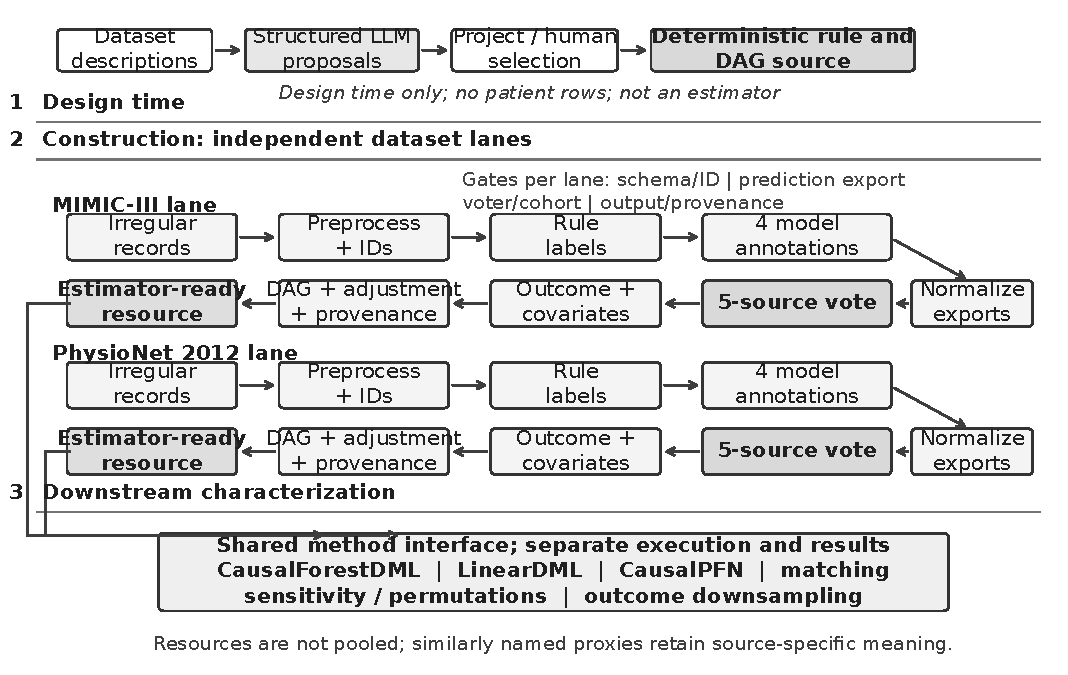
\includegraphics[width=0.99\textwidth]{figures/figure1_pipeline.pdf}
  \caption{CliniCause construction. Separate dataset lanes combine deterministic
  proxy rules and four normalized model annotations, then package five-source
  aggregates with outcomes, covariates, graph metadata, and provenance.
  Validation gates protect each handoff. The LLM proposes candidates only at
  design time; selected deterministic source governs runtime.}
  \label{fig:pipeline}
\end{figure*}

\subsection{Source Cohorts and Analysis Units}

The resources originate from MIMIC-III and the PhysioNet/Computing in Cardiology
Challenge 2012 collection \cite{johnson2016mimiciii,silva2012physionet}. An
analysis unit is a source time-series record or ICU stay, not necessarily a
unique person. Source identifiers map to a canonical \texttt{ts\_id}; irregular
events retain time, variable, and value, while a record table supplies mortality
and available baseline covariates. Linked long-event and record-level views
support temporal modeling and causal analysis without flattening irregular
events into the estimator table prematurely. Split-aware predictive artifacts
and the complete admitted causal cohort remain distinct and are aligned by
validation contracts rather than treated as interchangeable files.

The admitted populations contain 26,845 MIMIC-III and 7,993 PhysioNet records.
Their covariates, measurement processes, proxy ontologies, and graphs remain
dataset specific, so records and estimates are never pooled and similarly named
constructs are not assumed equivalent. The common interface standardizes
analytical roles---identifier, exposure, outcome, covariate, adjustment, and
provenance---rather than forcing a common clinical vocabulary onto the two
sources. Portability can therefore be evaluated without erasing source-specific
measurement and construct boundaries.

\begin{table*}[t]
  \centering
  \small
  \begin{tabular}{@{}p{0.11\textwidth}p{0.10\textwidth}p{0.095\textwidth}p{0.12\textwidth}p{0.20\textwidth}p{0.22\textwidth}@{}}
    \toprule
    Dataset & Records & Exposures & Outcome & Predictive annotations & Causal-analysis estimators \\
    \midrule
    MIMIC-III & 26,845 & 9 & In-hospital mortality & 1 rule source + 4 models & CF-DML, LinearDML, CausalPFN \\
    PhysioNet 2012 & 7,993 & 10 & In-hospital mortality & 1 rule source + 4 models & CF-DML, LinearDML, CausalPFN \\
    \bottomrule
  \end{tabular}
  \caption{Primary original-sampling resources. Counts are analysis records and
  admitted non-chronic proxy exposures, not raw cohorts; CF-DML denotes
  CausalForestDML.}
  \label{tab:resources}
\end{table*}

\subsection{Proxy-State Design and Deterministic Construction}

Before patient-level execution, a structured LLM protocol proposed proxy
ontologies, binary-rule families, missingness considerations, and dataset-
specific graphs. Project-selected proposals were encoded in deterministic tagger
and graph source. That source, not prompt text, governs runtime; the LLM neither
processes patient records nor assigns exposures or estimates effects. This
boundary makes proposals inspectable while ensuring that patient-level execution
depends on versioned deterministic artifacts.

Dataset-specific rules map measurements and care-process indicators to binary
proxy fields while preserving source differences (e.g., combined MIMIC-III
hepatic/coagulation evidence versus separate PhysioNet constructs). Missing
numeric measurements provide no positive rule evidence, making availability
part of construct provenance. These are transparent analytical proxies, not
chart-adjudicated diagnoses. Their explicit columns provide a replaceable
interface: reviewers can revise a rule without silently changing the outcome,
covariates, or cohort contract. Missing measurements cannot create positive rule
evidence by being silently interpreted as normal; the observed input envelope
remains part of each proxy's meaning.

\subsection{Predictive Annotations from Irregular Time Series}

Each predictive task estimates its dataset's rule-derived proxy vector. STraTS
represents sparse observation times, values, and variables; GRU and TCN process
temporal grids; and GRU-D models decay from missingness and time gaps
\cite{tipirneni2022strats,cho2014gru,bai2018tcn,che2018grud}. Static covariates
join each temporal representation. Value, observation-mask, and elapsed-time
channels preserve different aspects of irregular sampling across architectures.
Targets are proxy states, not mortality.

Normalized exports pair target probabilities with binary predictions at the
implemented 0.5 threshold. Archived causal runs combine one rule-derived source
and four aligned model sources by deterministic majority vote. This aggregate
is an algorithmic proxy-exposure layer, not a learned label model or expert
consensus. Predictive metrics characterize recovery of rule targets, not their
clinical validity. Probability and binary fields remain paired in normalized
exports, while aggregation consumes only aligned binary voters; prediction
evaluation therefore remains distinct from exposure assembly. Complete voter
sets are required so that a missing model export cannot silently change the
aggregation denominator or admitted cohort.

\subsection{Causal-Analysis Schema and DAG Metadata}

Estimator-ready rows align canonical identifiers, aggregate proxy fields,
in-hospital mortality, and source-specific covariates. Linked metadata records
dataset, sampling condition, graph, run, and artifact provenance. The analysis
admits nine non-chronic MIMIC-III and ten non-chronic PhysioNet exposures;
chronic-burden fields remain baseline constructs rather than analyzed
exposures. Exposure, outcome, adjustment, and provenance roles are explicit even
when their fields reside across linked tables and metadata.

For each exposure, a source-coded graph maps project assumptions to observed
columns and an exposure-specific adjustment set. The graphs are neither learned
nor clinically validated ground truth, but encoding them makes adjustment
choices inspectable and replaceable alongside proxies and estimators without
rebuilding source-data integration. Alternative graphs can consequently be
compared against the same aligned resource instead of being conflated with a
new preprocessing population. Graph or estimator changes thus remain visible
analytical choices rather than hidden changes to the data resource.

\subsection{Dataset Validation and Provenance}

Structural validation checks files, column order, identifiers, values, and
output completeness. Cohort contracts require identifier preservation and exact
equality at handoffs, rejecting duplicates, conflicts, missing or extra records,
and silent shrinkage. Unexpected columns, invalid voter/probability fields,
binary inconsistencies, and incomplete artifact sets fail explicitly. Together,
these checks protect one analytical population from deterministic labels through
predictive annotations and estimator-ready assembly.

Validation also spans artifact identity and execution boundaries. Prediction,
checkpoint, and voter sidecars bind model and input roles; run receipts
distinguish planned from completed stages; upstream fingerprints prevent reuse
after source mutation; and dataset-isolated paths prevent cross-source artifact
substitution. A handoff is validated only when its required evidence is present,
rather than inferred from a file name or partial directory.

Artifact validation binds outputs to supported metadata, hashes, schemas,
cohorts, configurations, and seeds. Dataset-isolated run paths, manifests,
receipts, and sidecars record roles and outputs; stale or mutation-mismatched
artifacts fail reuse checks. Deterministic transformations and derived seeds
avoid dependence on ambient order or process state. These contracts concern the
current resource interface and do not recover historical run provenance by
themselves.

The checked archive establishes valid export schemas, complete primary
aggregates, manifests, checksums, and archived analysis-stage records, but exact
producing revisions, configurations, and checkpoint-to-export links remain
incomplete. The repaired current code contains stricter source/test contracts;
it is not claimed as the historical producer, nor do we claim current test
execution. Keeping these evidence layers separate avoids turning checked output
integrity into an unsupported exact-rerun claim.

Both resources supported predictive characterization, three effect estimators,
graph-guided adjustment, matching, and robustness diagnostics. Validation thus
establishes structural integrity, cohort consistency, provenance, and analytical
reuse; clinical construct validity and causal identification remain separate
questions. This scoped definition permits strong resource validation without
promoting proxy states to diagnoses or adjusted contrasts to proven effects.
For current-code reproduction, one top-level launcher exposes dedicated
dataset-construction and complete-pipeline modes. The supplement documents the
Python 3.10 environment, single dependency installation, authorized data paths,
validation, manifests, receipts, and provenance needed to reconstruct the
derived resources; missing producing lineage still precludes a verified
historical rerun, and an approved anonymous repository location remains gated.

\section{Empirical Evaluation}
% P4 claim locations: C02, C05, C08, C14--C16, C19, C28, C39, and C41--C55
% in paper_evidence_map.md. Numerical findings remain reserved for Section 5.

The evaluation asks three linked questions. First, can irregular-time-series
models recover the constructed rule targets, and does their behavior differ by
dataset? Second, are the principal exposure--outcome directions stable across
distinct estimator forms? Third, do matching and population perturbations expose
support or sign sensitivity? These questions characterize the resources and
their analytical interfaces; they do not test a clinical intervention.

\subsection{Prediction Tasks and Metrics}

For each dataset, STraTS, GRU, GRU-D, and TCN predict its deterministic proxy
vector. We compare one selected archived held-out test output per model--dataset
combination, without pooling targets or scores. Because repeated-run uncertainty
is unavailable, these point metrics characterize prediction of rule-derived
constructs, not statistical superiority or clinical validity. Target sets follow
the source-specific schemas, so the evaluation asks whether each constructed
proxy vector can be recovered from its own irregular ICU representation.
The comparison includes all eight archived model--dataset outputs selected for
the main analysis rather than choosing models by a single favorable metric.

We report sample-mean multi-label binary cross-entropy loss and macro AUROC,
AUPRC, and minRP. Per target, minRP maximizes the smaller of precision and recall
over thresholds. The three discrimination scores are averaged after excluding
single-class targets; loss follows the archived sample-mean evaluator output.
No confidence interval or significance test is inferred from the selected runs.

\subsection{Effect Estimators and Cross-Estimator Evaluation}

Each admitted aggregate proxy is analyzed separately as a binary exposure,
with in-hospital mortality as outcome and observed adjustment variables selected
by the project graph. Every prespecified non-chronic exposure is retained. The
original populations are primary, and datasets are analyzed without pooling.
This complete-set policy prevents favorable post-hoc exposure selection. The
graphs encode the project's observed-adjustment assumptions; they do not remove
requirements for consistency, overlap, well-defined interventions, or absence
of unmeasured confounding.

CausalForestDML is the primary nonlinear estimator, combining DML adjustment
with a causal-forest final stage \cite{chernozhukov2018dml,wager2018causalforest,
athey2019grf,oprescu_et_al_2019_econml} to obtain record-level fitted conditional
effects. LinearDML retains the DML nuisance framework with a linear final effect
model, isolating a change in final-stage form. CausalPFN
\cite{balazadeh2025causalpfn} provides a distinct complementary paradigm over
the same prespecified comparisons; its archived estimator-specific sensitivity
and permutation coverage is less complete than for DML.

We summarize fitted conditional estimates by their \emph{mean model-estimated
CATE over the analyzed sample}, not as a risk ratio, odds ratio, or unqualified
population ATE. We compare its sign between the DML estimators and across all
three estimators, retaining disagreements. Directional agreement neither
requires equal magnitudes nor proves causal identification; it tests whether the
principal sign pattern depends on one estimator family. All interpretations are
therefore observational and proxy based, and none is a treatment recommendation.
Magnitude remains visible in Figure~\ref{fig:agreement} so sign concordance does
not collapse substantively different fitted summaries into equivalence.

\subsection{Matching and Robustness Diagnostics}

Matching is a descriptive support check: binary adjustment variables and
median-binarized numeric variables enter greedy one-to-one Hamming matching.
The procedure begins with exact binary matches and increases allowed distance
within its configured pair-count and match-rate criteria. We report a
\emph{descriptive matched-pair outcome difference} with availability, distance,
and support warnings; no usable representation produces an explicit failure,
not a zero effect or an imputed estimate.

Archived DML sensitivity records retain native, recomputed/reconstructed,
partial, failed, and unavailable provenance classes. Treatment and outcome
permutations are disruption checks rather than formal randomization tests or
identification proofs. Equivalent stages were not archived for CausalPFN, which
marks diagnostic-coverage asymmetry rather than exclusion from triangulation.
For DML, recorded sensitivity provenance is preserved because estimator-native,
later reconstructed, partial, and failed evidence are not interchangeable forms
of validation.

Outcome downsampling retains mortality-positive records and samples negatives,
changing both population and prevalence. It is a robustness perturbation, not a
co-primary analysis, and its magnitudes are not interchangeable with original-
population estimates. Applying the shared sequence separately to both resources
tests workflow portability while preserving dataset-specific definitions,
cohorts, and causal assumptions. The matching, disruption, and downsampling
analyses are supporting diagnostics; no single check upgrades adjusted
observational contrasts into identified intervention effects.

\section{Results}

The resources comprise 26,845 MIMIC-III records with nine exposures and 7,993
PhysioNet records with ten. All analyses remain dataset specific and unpooled.

\subsection{Predictive Characterization}

STraTS led all four archived MIMIC-III point metrics, whereas GRU-D led all four
PhysioNet metrics (Table~\ref{tab:predictive-results}). This dataset-dependent
leadership does not imply statistical superiority. STraTS reached 0.905 AUROC
and 0.869 AUPRC on MIMIC-III; GRU-D reached 0.918 and 0.905 on PhysioNet. Each
also led loss and minRP within its dataset, so leadership was consistent across
the four archived metrics against rule-derived targets. The change in leader
reinforces the resource design choice to retain source-specific measurement and
missingness semantics rather than select one temporal representation globally.

\begin{table*}[!t]
  \centering
  \small
  \begin{tabular}{@{}llrrrr@{}}
    \toprule
    Dataset & Model & Test loss$\downarrow$ & Test AUROC$\uparrow$ & Test AUPRC$\uparrow$ & Test minRP$\uparrow$ \\
    \midrule
    MIMIC-III & STraTS & \textbf{0.348} & \textbf{0.905} & \textbf{0.869} & \textbf{0.795} \\
    & GRU & 0.386 & 0.881 & 0.840 & 0.770 \\
    & GRU-D & 0.404 & 0.884 & 0.841 & 0.773 \\
    & TCN & 0.414 & 0.867 & 0.823 & 0.758 \\
    \addlinespace
    PhysioNet 2012 & STraTS & 0.341 & 0.915 & 0.877 & 0.818 \\
    & GRU & 0.397 & 0.915 & 0.897 & 0.831 \\
    & GRU-D & \textbf{0.331} & \textbf{0.918} & \textbf{0.905} & \textbf{0.835} \\
    & TCN & 0.477 & 0.899 & 0.875 & 0.811 \\
    \bottomrule
  \end{tabular}
  \caption{Selected archived held-out point metrics against rule-derived proxy
  targets. Bold marks each dataset's best value; no significance is implied.}
  \label{tab:predictive-results}
\end{table*}

\subsection{Effect Patterns and Estimator Agreement}

All nine MIMIC-III CausalForestDML mean summaries were positive, as were nine of
ten PhysioNet summaries. MIMIC-III was led by cardiac strain (0.220) and
inflammation/sepsis (0.161); PhysioNet was led by renal dysfunction (0.120),
cardiac injury/strain (0.112), and global severity (0.108), while shock was
negative ($-0.014$). These are mean model-estimated CATE over the analyzed
samples under the implemented proxy and adjustment design; magnitudes and
construct orderings remained dataset specific (Figure~\ref{fig:agreement}).

CausalForestDML and LinearDML agreed in direction for all 19 prespecified
comparisons. CausalPFN joined their direction in 18/19, providing triangulation
from a distinct modeling paradigm while retaining its smaller archived
diagnostic envelope. Complete DML concordance shows that the sign pattern was
not unique to a linear or forest final stage, while CausalPFN's broad agreement
extends the observation beyond that shared DML framework. Neither result implies
equal magnitudes or identifies a causal effect.

PhysioNet shock was the sole exception: CausalForestDML was $-0.014$, LinearDML
$-0.027$, and CausalPFN 0.004; its descriptive matched-pair difference was
0.010. The disagreement motivates targeted analysis of the proxy, support,
adjustment assumptions, and estimator behavior rather than estimator voting.
Retaining this near-zero exception is important because a direction-only summary
would otherwise conceal exactly where model choice changes the conclusion.

\begin{figure*}[!t]
  \centering
  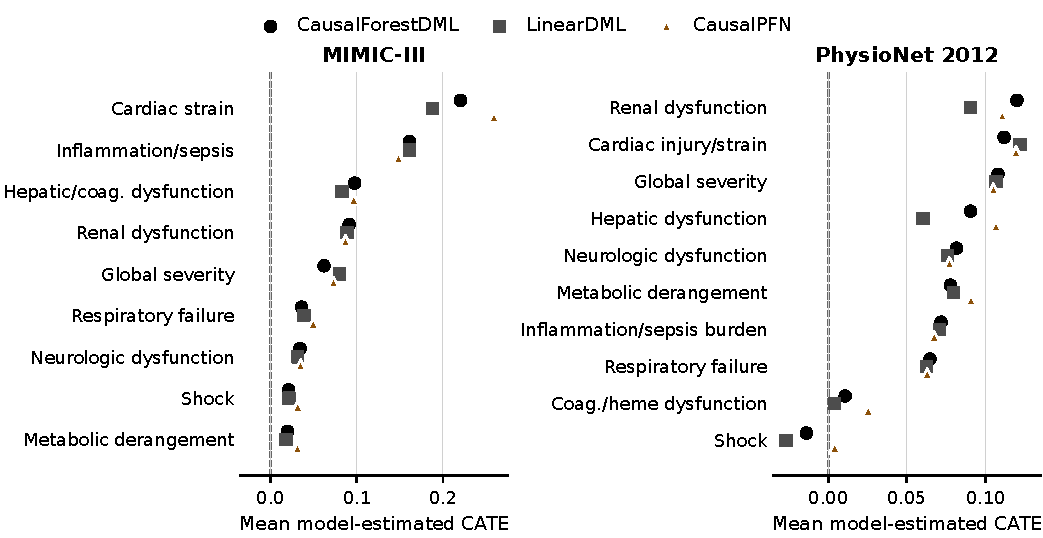
\includegraphics[width=0.99\textwidth]{figures/figure2_estimator_agreement.pdf}
  \caption{All 19 original-cohort comparisons, ordered by CausalForestDML.
  Markers are mean model-estimated CATE over each analyzed sample. DML directions
  agree in 19/19 and all three in 18/19; PhysioNet shock is the exception.}
  \label{fig:agreement}
\end{figure*}

\subsection{Robustness and Cross-Dataset Findings}

Matching succeeded for 15/19 comparisons (eight MIMIC-III and seven PhysioNet);
four failures lacked usable binary columns and are not zero effects. Of the 15
summaries, 14 agreed with the primary direction; PhysioNet shock did not.
The availability split also distinguishes empirical support limitations from
estimator disagreement on completed analyses. Matching agreement is descriptive
corroboration only: it neither repairs failed overlap nor supplies an independent
identified causal effect.

Direction persisted in 55/57 original-versus-downsampled comparisons. The two
changes were PhysioNet LinearDML coagulation/hematologic dysfunction and
PhysioNet CausalPFN shock; magnitudes do not transport to the original
population. DML sensitivity and permutation evidence has nonuniform provenance
and coverage, with no equivalent archived CausalPFN stages; these diagnostics
remain supporting evidence rather than independent identification tests.
Together, differing predictive leaders and effect patterns alongside broad
estimator agreement show workflow portability, not pooled clinical replication.

\FloatBarrier
\section{Discussion and Limitations}

\subsection{Resource Utility and Cross-Dataset Portability}

CliniCause contributes reusable resources rather than only effect tables.
Explicit exposure, outcome, covariate, graph, cohort, and provenance interfaces
support comparisons of estimators and temporal representations without repeating
every integration stage. Deterministic definitions and lineage also make proxy,
graph, adjustment, cohort, and support alternatives directly auditable. A study
can replace one layer while retaining the remaining analytical contract, making
the present estimates starting points for controlled follow-up rather than
fixed endpoints. Concretely, the same tables can support estimator benchmarking;
the event-to-proxy interface can test new temporal representations; and preserved
construct and graph metadata can support clinician-led proxy or adjustment
revision. Each use keeps cohort identity visible, helping distinguish a method
change from an unnoticed population change.
Because resource validation is separated from clinical and causal validation,
follow-up studies can strengthen one evidence layer without discarding the
audited interfaces already established in the others.

The validation contracts are scientifically consequential rather than only
software safeguards. Exact cohort equality prevents a join from silently
changing the population summarized by an estimator. Schema and voter checks
prevent missing annotations from redefining an exposure. Graph and adjustment
metadata expose assumptions that would otherwise be implicit, while hashes and
receipts distinguish a known artifact from a similarly named replacement.
Together these controls make differences between analyses attributable to
declared choices instead of undetected pipeline drift. They do not establish
that a proxy or graph is correct, but they make those scientific questions
answerable on a stable resource.

The same sequence operated across heterogeneous ICU sources although predictive
leadership, magnitudes, and rankings differed. Portability therefore resides in
the workflow and interface, not construct equivalence: variables, measurement
processes, ontologies, graphs, and analyses remain dataset specific and unpooled.
This separation exposes contextual sensitivity instead of hiding it behind a
pooled replication claim. It also lets future work distinguish success of a
common interface from equivalence of source semantics. Operation on two sources
demonstrates workflow portability, not external clinical generalization of any
proxy or effect estimate.
The source differences also illustrate why a common interface is preferable to
a forced common ontology. MIMIC-III and PhysioNet vary in available variables,
sampling processes, and whether hepatic and coagulation evidence form one proxy
or two. Preserving those differences allows researchers to compare methods while
tracing disagreement to representation, construct, adjustment, support, or
estimator choices. A pooled table would make that attribution harder and could
give similarly named columns a false clinical equivalence.

\subsection{Estimator Triangulation and CausalPFN}

The 19/19 DML and 18/19 all-estimator sign agreements show that the prevailing
pattern extends across final-stage forms and to CausalPFN's distinct paradigm.
PhysioNet shock usefully exposes model and support sensitivity for targeted
study. Directional agreement does not establish equal magnitudes, uncertainty,
or causal identification; CausalPFN's smaller archived diagnostic envelope
also motivates estimator-specific follow-up. Broad concordance plus one visible
exception is more informative than an aggregate vote: it supports further
CausalPFN evaluation while identifying a concrete case for proxy, adjustment,
overlap, and estimator analysis.
For future estimator studies, the complete 19-comparison matrix supplies both a
broad concordance target and a prespecified stress case. Repeated runs,
estimator-specific uncertainty, and harmonized diagnostics should determine
whether the shock disagreement is sampling variation, weak support, construct
sensitivity, or a genuine modeling difference.

\subsection{LLM-Assisted Design and Future Research}

The LLM layer is a design aid for inspectable proxy, missingness, and graph
proposals; project selection and deterministic source retain authority. Future
work can use the resources to test clinician-reviewed proxies, expert/LLM or
design-layer alternatives, graphs, repeated-run uncertainty, richer CausalPFN
diagnostics, and external datasets. Because proposals remain separate from
patient execution, such comparisons need not grant the LLM runtime clinical
authority. Prompt sensitivity and proposal-to-source traceability should also be
evaluated so that any design benefit is distinguishable from downstream human
selection and deterministic implementation.

\subsection{Limitations}

Proxy states are analytical constructs, not chart-adjudicated phenotypes, but
their definitions and lineage permit clinician-led replacement and validation.
Project graphs do not prove intervention validity; observational estimates
remain vulnerable to unmeasured confounding, identification, and support
failures and are not treatment recommendations. Alternative graphs, adjustment
sets, and stronger support analyses are necessary before stronger
interpretation. Repeated-run uncertainty and diagnostic coverage are incomplete,
especially for CausalPFN. Exact producing
revisions, configurations, and checkpoint-to-export lineage also remain
incomplete; current runtime and anonymous release are separately gated.
Accordingly, archived point-metric leaders are not statistical rankings, the
agreement counts are not uncertainty estimates, and the present artifacts do
not support an exact clean-checkout reproduction claim.
Restricted source-data access, absent external clinical validation, and no
isolated LLM ablation further limit generalization. The resource interfaces make
these boundaries explicit and testable rather than burying them in undocumented
pipeline choices. Replaceability facilitates those studies but is not itself
evidence that a replacement, proxy, or graph is clinically valid.

\section{Conclusion}

CliniCause constructs reusable, estimator-ready resources from MIMIC-III and
PhysioNet 2012 with validated structural, cohort, provenance, and analytical
interfaces. Broad DML/CausalPFN directional agreement demonstrates bounded
estimator triangulation: the DML estimators agreed in 19/19 directions and
CausalPFN joined them in 18/19, with PhysioNet shock retaining the informative
exception. Archived predictive leadership also differed by dataset, reinforcing
the need to preserve source semantics. These transparent resources support tests
of proxy definitions, temporal representations, graphs, cohorts, and estimators
while preserving the observational and proxy-based boundary of the findings.
This foundation is intended for transparent comparison and revision, not
patient-level deployment or treatment selection. Its value lies in making the
next proxy, graph, representation, or estimator comparison easier to specify,
audit, and interpret.

% The approved repository bibliography is connected without copying or editing
% it. No citation is rendered until its exact use is evidenced and drafted.
\bibliography{../literature/metadata/references}

% AAAI-27 requires the reproducibility checklist as a separate submission-field
% upload. Do not \input or append AuthorKit27/ReproducibilityChecklist.tex here.

\end{document}
